\documentclass[11pt,letterpaper]{article}
\PassOptionsToPackage{hyphens}{url}
\usepackage[margin=.83in,top=.8in,bottom=.8in,headheight=15pt]{geometry}
\usepackage[T1]{fontenc}
\usepackage{lmodern,amsmath,amssymb,mathtools,bm,booktabs,array,graphicx,tikz}
\usetikzlibrary{arrows.meta,positioning,calc,decorations.pathreplacing,patterns}
\definecolor{ink}{HTML}{17344D}\definecolor{accent}{HTML}{087E8B}\definecolor{pale}{HTML}{EDF5F5}\definecolor{gold}{HTML}{AD6B19}
\providecommand{\dd}{\,\mathrm{d}}\providecommand{\R}{\mathbb{R}}
\providecommand{\E}{\mathbb{E}}\providecommand{\Var}{\operatorname{Var}}
\providecommand{\Cov}{\operatorname{Cov}}\providecommand{\diag}{\operatorname{diag}}
\providecommand{\norm}[1]{\left\lVert#1\right\rVert}
\providecommand{\abs}[1]{\left|#1\right|}
\usepackage{microtype,hyperref,fancyhdr,enumitem,amsthm,sectsty,needspace}
\allsectionsfont{\raggedright}
\hypersetup{colorlinks=true,linkcolor=ink,urlcolor=accent,pdfauthor={Zan Ahmad},pdftitle={Pulsatile circulation: changing compliance and self-consistent valves / Lecture notes}}
\setlength{\parindent}{0pt}\setlength{\parskip}{6pt}\linespread{1.07}
\setlist{itemsep=3pt,topsep=4pt,leftmargin=*}
\emergencystretch=2em\clubpenalty=10000\widowpenalty=10000
\pagestyle{fancy}\fancyhf{}\fancyhead[L]{\small Mathematical Modeling}\fancyhead[R]{\small Lecture 4}
\fancyfoot[L]{\footnotesize Zan Ahmad}\fancyfoot[R]{\footnotesize\thepage}\renewcommand{\headrulewidth}{.3pt}
\newtheorem{proposition}{Proposition}\newtheorem{theorem}{Theorem}\newtheorem{lemma}{Lemma}
\theoremstyle{definition}\newtheorem{definition}{Definition}\newtheorem{example}{Example}
\numberwithin{equation}{section}
\begin{document}
{\small\scshape Mathematical Modeling\hfill Lecture 4}\par\medskip
{\raggedright\hyphenpenalty=10000\exhyphenpenalty=10000\LARGE\bfseries\color{ink} Pulsatile circulation: changing compliance and self-consistent valves\par}\medskip
{\small Lecture notes}\par\bigskip
A pump changes pressure while redistributing a conserved volume. We combine compliant storage, resistive flow, and ideal one-way valves in a six-compartment circuit. Differentiating the storage relation produces a product derivative. Its numerical solution requires two nested tasks: advancing physical time and finding valve states consistent with the new pressures. The companion runs a fixed-rate baseline; it does not run a feedback controller.

\section{Six compartments and a closed volume account}
\hypertarget{note-six-compartments-and-a-closed-volume-account}{}\label{note:six-compartments-and-a-closed-volume-account}
{\small \href{slides.html\#frame=conservation-storage-and-link-laws\&step=1}{Slides for this section}}\par
Order the stores as LV, systemic artery (SA), systemic vein (SV), RV, pulmonary artery (PA), and pulmonary vein (PV). The directed valves connect PV to LV, LV to SA, SV to RV, and RV to PA. Open tissue resistances connect SA to SV and PA to PV. They allow signed flow in either direction.

Let $t$ measure time in seconds and $\tau=t/60$ time in minutes. In the hydraulic differential equations below, a dot denotes differentiation with respect to $\tau$, so $\dot V$ is in L/min. An incidence matrix $B$ places $-1$ at each link's source and $+1$ at its destination. Thus $\dot{\mathbf V}=B\mathbf Q$ and $\mathbf1^TB=0$ imply $\dd\sum_iV_i/\dd\tau=0$. This result uses the closed topology, not an assumption that each component volume is steady. Functional compartments collect many physical vessels; the model contains no external fluid input.

Pressure is in mmHg, volume in L, compliance in L/mmHg, and flow in L/min. A timestep supplied in seconds must be divided by $60$ in a hydraulic balance. The baseline uses $80$ beats/min, a $15$ s startup interval, and systemic resistance $17.86\ \mathrm{mmHg}\,\mathrm{min}/\mathrm L$. The reference circulation code used $8$. Their trajectories are not the same parameter experiment.
\section{Pumping by a time-dependent storage relation}
\hypertarget{note-pumping-by-a-time-dependent-storage-relation}{}\label{note:pumping-by-a-time-dependent-storage-relation}
{\small \href{slides.html\#frame=shared-ventricular-phase\&step=1}{Slides for this section}}\par
In each compartment,
\[
V_i=V_{d,i}+C_i(t)P_i,\qquad C_i>0,
\]
where $V_{d,i}$ is a constant unstressed volume. Vascular compliances are fixed; the two ventricular compliances vary with a shared phase. With $t$ in seconds and fixed rate $f$ in beats/min, $\phi=f\tau=ft/60$ cycles. A waveform periodic in phase has period $T=60/f$, or $0.75$ s at $80$ beats/min.

Using the minute-time derivative defined above, the product rule is
\[
\dot V_i=C_i\dot P_i+\dot C_iP_i.
\]
With closed valves and fixed volume, $C_iP_i$ is constant, so $\dot P_i=-(\dot C_i/C_i)P_i$. Decreasing compliance raises pressure without adding fluid. If $V-V_d=0.10$ L and $C=0.002$ L/mmHg, then $P=50$ mmHg; halving $C$ at fixed volume doubles $P$.

Changing compliance supplies the prescribed actuation. Valves direct the resulting flow but do not create energy. The model has neither myocardial stress nor a three-dimensional wall deformation; those require further variables and constitutive relations.
\section{Valve flow and the pressure inequalities}
\hypertarget{note-valve-flow-and-the-pressure-inequalities}{}\label{note:valve-flow-and-the-pressure-inequalities}
{\small \href{slides.html\#frame=ideal-valve-inequalities\&step=1}{Slides for this section}}\par
For a valve with upstream and downstream pressures, define
\[
Q=G[P_{\rm up}-P_{\rm down}]_+,\qquad[z]_+=\max(z,0),\qquad G=1/R.
\]
An open candidate requires $P_{\rm up}\geq P_{\rm down}$; a closed candidate requires $P_{\rm up}\leq P_{\rm down}$ and gives zero flow. At equality both limiting descriptions yield zero flow. An ordinary resistor instead uses $Q=G(P_{\rm up}-P_{\rm down})$ without a direction constraint.

As a hand calculation, $110-90=20$ mmHg across $R=2\ \mathrm{mmHg}\,\mathrm{min}/\mathrm L$ gives $10$ L/min. A $0.06$ s interval transfers $10(0.06/60)=0.010$ L, or $10$ mL. Subtract and add precisely that transfer at the two endpoints. Reversed pressure closes the valve but reverses an open-resistor flow.
\section{An implicit equation for pressure}
\hypertarget{note-an-implicit-equation-for-pressure}{}\label{note:an-implicit-equation-for-pressure}
{\small \href{slides.html\#frame=backward-difference-of-stored-volume\&step=1}{Slides for this section}}\par
Write $C^n=\operatorname{diag}(C_i^n)$, and let $h$ be in minutes. For a fixed candidate set of open valves, form the symmetric Laplacian $L_S$: diagonal entries sum active incident conductances and off-diagonal entries are their negatives. Backward Euler in stored volume is
\[
\frac{C^{n+1}\mathbf P^{n+1}-C^n\mathbf P^n}{h}=-L_S\mathbf P^{n+1}.
\]
The constant unstressed volumes cancel. Collecting the unknown pressures gives
\[
\boxed{(C^{n+1}+hL_S)\mathbf P^{n+1}=C^n\mathbf P^n.}
\]
Replacing the numerator by $C^{n+1}(\mathbf P^{n+1}-\mathbf P^n)$ would omit the effect of changing compliance. Likewise, reconstructing a volume using pressure and compliance from different phases violates the storage law.

For nonzero $\mathbf z$,
\[
\mathbf z^T(C^{n+1}+hL_S)\mathbf z=\sum_i C_i^{n+1}z_i^2+h\sum_{\{i,j\}\ {\rm active}}G_{ij}(z_i-z_j)^2>0.
\]
Thus every fixed-state linear system is invertible. This does not establish consistency of the guessed valve states. Implicit treatment handles the fast equilibration produced by low valve resistance without the severe explicit stability restriction, but timestep accuracy remains a separate question.
\section{A complete valve-state iteration}
\hypertarget{note-a-complete-valve-state-iteration}{}\label{note:a-complete-valve-state-iteration}
{\small \href{slides.html\#frame=nested-time-and-valve-iterations\&step=1}{Slides for this section}}\par
Hold $\mathbf P^n$, both compliance vectors, and $h$ fixed. Guess four valve states, solve the corresponding pressure system, test the pressure inequalities, and revise the guess if necessary. Repeated candidate solves occur within one physical timestep.

A two-compartment reduction provides a numerical trace in consistent scaled units. Take $C^{\rm old}=(1,1)$, $P^{\rm old}=(2,1)$, $C^{\rm new}=(0.5,1)$, and $hG=1$. A closed guess for a valve $1\to2$ gives $(P_1,P_2)=(4,1)$, contradicting the closure inequality. The open candidate solves
\[
\begin{bmatrix}1.5&-1\\-1&2\end{bmatrix}
\begin{bmatrix}P_1\\P_2\end{bmatrix}=
\begin{bmatrix}2\\1\end{bmatrix},
\qquad (P_1,P_2)=(2.5,1.75).
\]
Now $P_1>P_2$, so the state is consistent. New stored amounts are $1.25$ and $1.75$, totaling the original $3$. The transfer is $hG(P_1-P_2)=0.75$.

The supplied algorithm bounds iterations, detects revisited guesses, and can enumerate all $2^4=16$ combinations. If no consistent admissible state is found, it raises an error rather than accepting the last candidate. The pressure/flow figure displays the corresponding full-model relation between LV and systemic arterial pressure and aortic valve flow.
\begin{center}\begin{minipage}{.98\linewidth}\centering
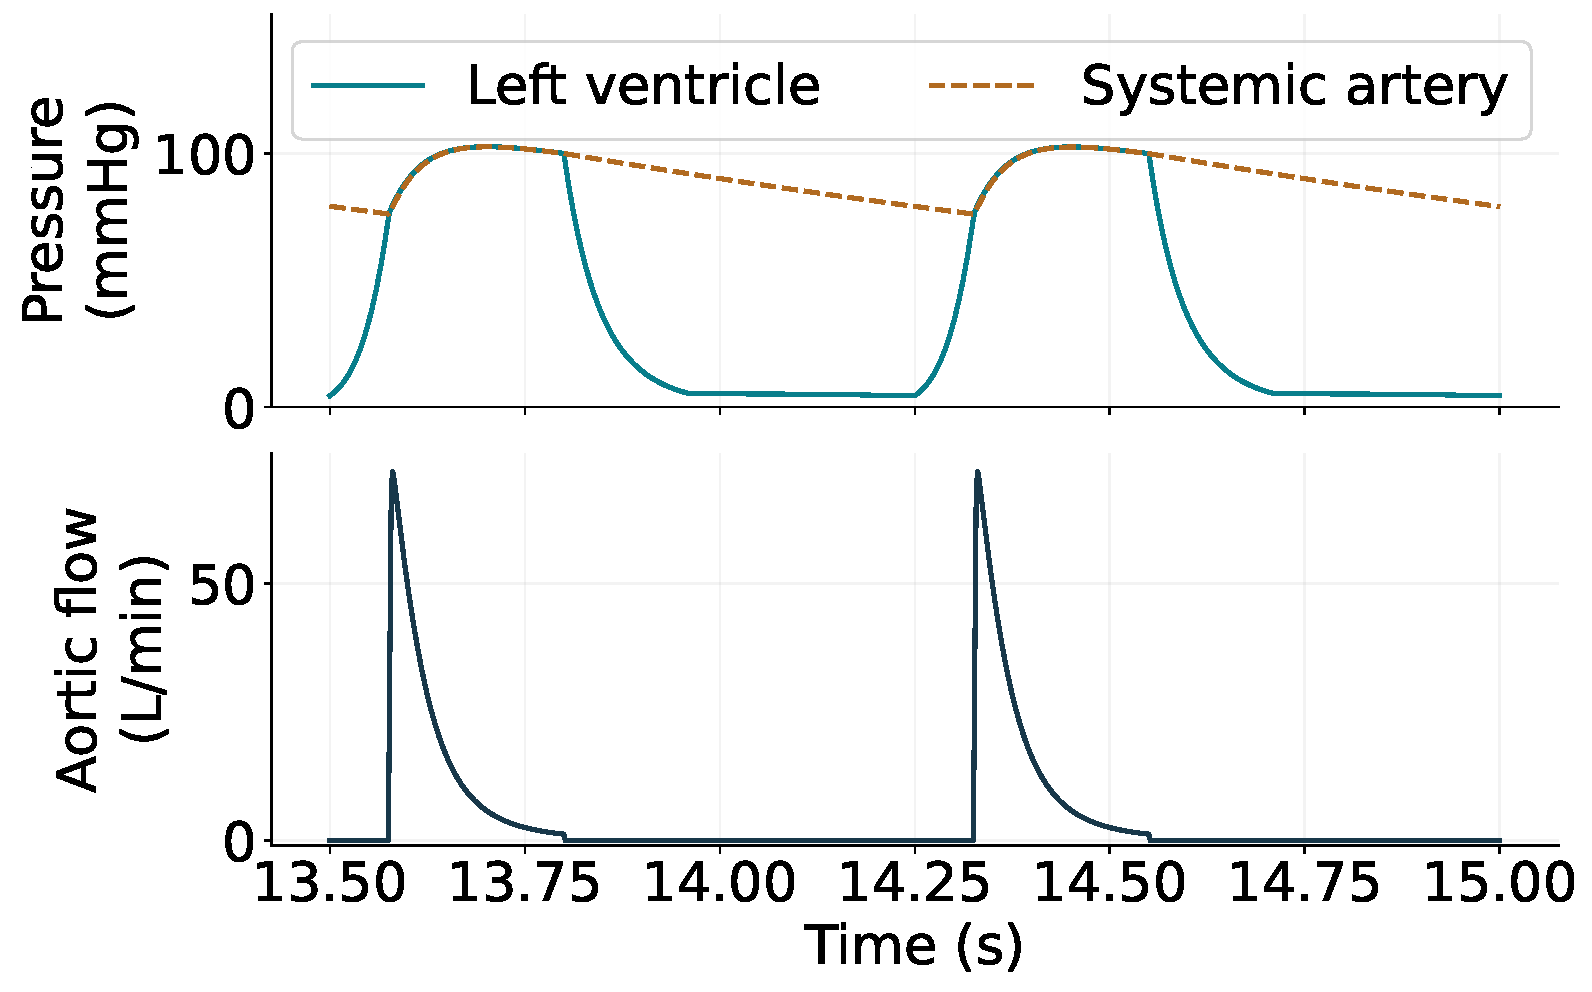
\includegraphics[width=.96\linewidth,height=.57\textheight,keepaspectratio]{presentation-figures/pressure-and-valve.pdf}\par\smallskip
{\small Final 1.5 seconds of the synthetic 15-second baseline, with fixed rate 80 beats/min. Aortic flow is positive only when ventricular pressure exceeds systemic arterial pressure.}
\end{minipage}\end{center}
\Needspace{10\baselineskip}
\section{Matched-state residuals and conservation}
\hypertarget{note-matched-state-residuals-and-conservation}{}\label{note:matched-state-residuals-and-conservation}
{\small \href{slides.html\#frame=discrete-total-volume-conservation-figure\&step=1}{Slides for this section}}\par
The figures show the final $1.5$ s of a $15$ s startup run. Positive aortic flow coincides with LV pressure exceeding SA pressure. Individual ventricular volumes change, while the six-region total stays at the initialized $5.13616$ L. This does not establish that the startup transient has ended.

Check the local residual using new flows,
\[
\mathbf r^{n+1}=\frac{\mathbf V^{n+1}-\mathbf V^n}{h}-B\mathbf Q^{n+1},
\]
and independently reconstruct $V_i^{n+1}=V_{d,i}+C_i(\phi_{n+1})P_i^{n+1}$. Since $\mathbf1^TL_S=0$, summing the implicit equation proves conservation of $\sum_iC_iP_i$, hence of total volume after adding fixed unstressed volumes. Conservation cannot alone certify valve direction, time accuracy, or biological validity.

Halving the step at fixed physical endpoint and inputs tests numerical sensitivity. Changing resistance or compliance tests a different model experiment. When resistance changes, recompute its reciprocal in both the pressure solve and flow output. Reusing an old conductance would make the two parts obey different laws. The existing numerical example supplies a study of this explicitly defined lumped model, not a calibrated clinical circulation.
\begin{center}\begin{minipage}{.98\linewidth}\centering
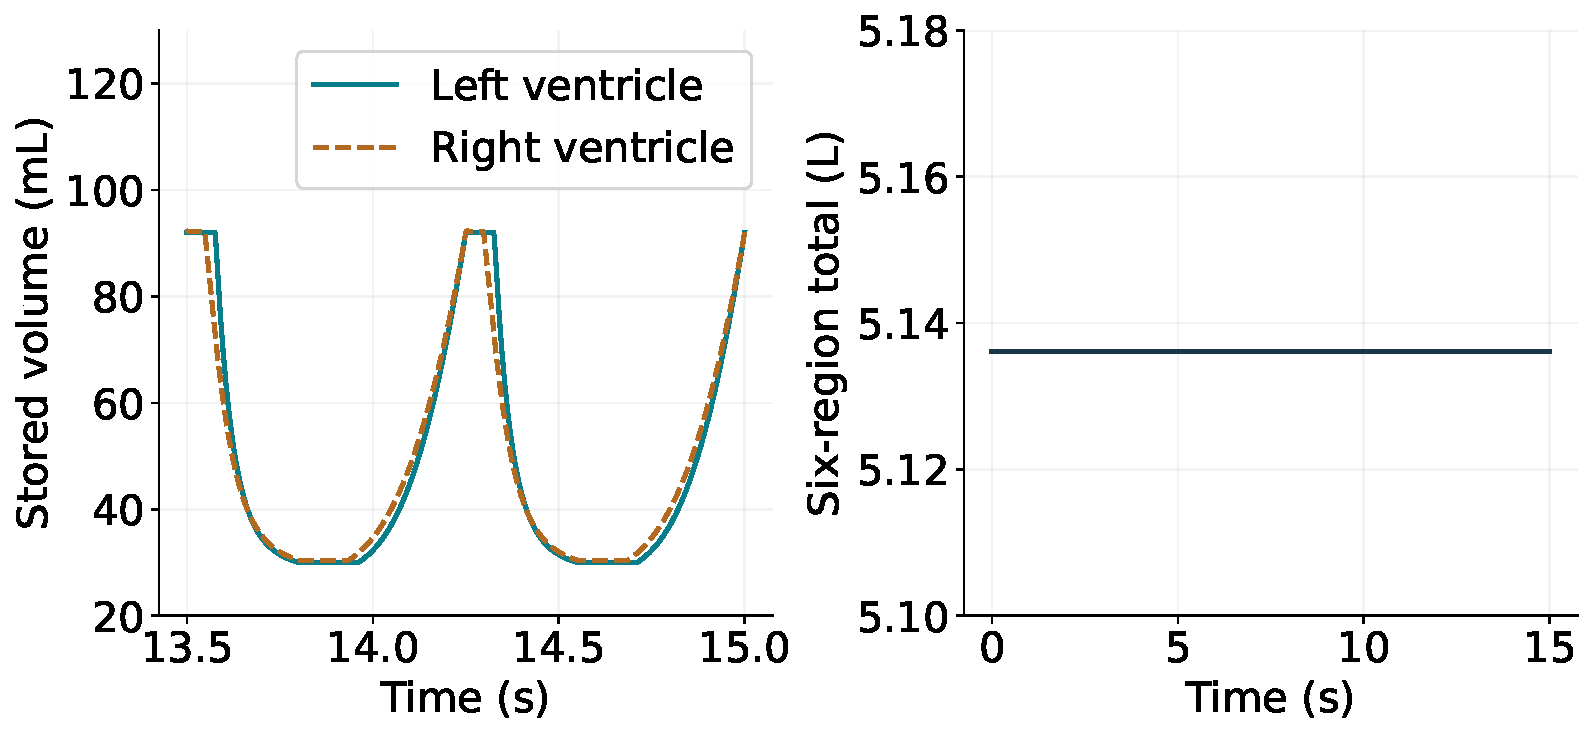
\includegraphics[width=.96\linewidth,height=.57\textheight,keepaspectratio]{changing-storage.pdf}\par\smallskip
{\small Ventricular volumes change over the final two nominal cycles; the sum of all six stored volumes stays at 5.13616 L across the entire 15-second calculation.}
\end{minipage}\end{center}
\bigskip
\section*{Exercises}
\par\noindent\begin{minipage}{\linewidth}
\subsection*{MM04-E1. Give one transfer two signs}
Two regions initially hold 300 mL and 500 mL. A forward valve has upstream pressure 100 mmHg, downstream pressure 80 mmHg and resistance 4 mmHg min/L.

\textbf{a} Compute the ideal forward flow.

\end{minipage}\par\medskip
\textbf{b} If that flow stays fixed for 0.12 s, compute the transfer and new volumes.

\textbf{c} Check the total and state what this calculation assumes.

\par\noindent\begin{minipage}{\linewidth}
\subsection*{MM04-E2. Change compliance without changing volume}
A sealed region has unstressed volume 30 mL, initial compliance 3 mL/mmHg and pressure 8 mmHg.

\textbf{a} Compute its total volume.

\end{minipage}\par\medskip
\textbf{b} Compliance falls to 1.5 mL/mmHg with no transfer. Find the required pressure.

\textbf{c} A program holds pressure at 8 mmHg after this change. Identify the inconsistency.

\par\noindent\begin{minipage}{\linewidth}
\subsection*{MM04-E3. Read a solver trace}
During one new time step, a candidate has a forward valve open but solved upstream pressure 70 mmHg and downstream pressure 85 mmHg.

\textbf{a} Should the candidate valve state be accepted?

\end{minipage}\par\medskip
\textbf{b} Why is setting the reported negative flow to zero after the solve insufficient?

\textbf{c} Name what changes and what stays fixed during this retry.

\par\noindent\begin{minipage}{\linewidth}
\subsection*{MM04-E4. Separate checks from model changes}
Run A uses a step of 0.002 s and resistance 18 mmHg min/L. Run B uses 0.001 s and the same resistance. Run C uses 0.001 s and resistance 9 mmHg min/L.

\textbf{a} Which comparison isolates time-step sensitivity, if initial state and final time are identical?

\end{minipage}\par\medskip
\textbf{b} What does B versus C investigate?

\textbf{c} If every run conserves total volume, does that validate all predicted pressures against a real circulation?

\section*{References}
\noindent\begin{minipage}{\linewidth}
Zan Ahmad, Fall 2024 HEART syllabus. PDF pages 1--2.

\end{minipage}\par\medskip
\noindent\begin{minipage}{\linewidth}
Hoppensteadt and Peskin, Modeling and Simulation in Medicine and the Life Sciences, second edition. Printed pages 48--51 and 55--58; supplied PDF pages 61--64 and 68--71.

\end{minipage}\par\medskip
\end{document}
